\section{INTRODUCTION}
A central goal in robotics is the execution of long-horizon tasks in
the face of uncertainty. Any reader that has spent frantic mornings
searching for lost keys understands the challenges such problems
present. Completing such a task corresponds to reasoning about
multimodal belief distributions where obtaining an observation
can require long, temporally extended plans. 
\begin{figure}[h]
  \centering
    \noindent
    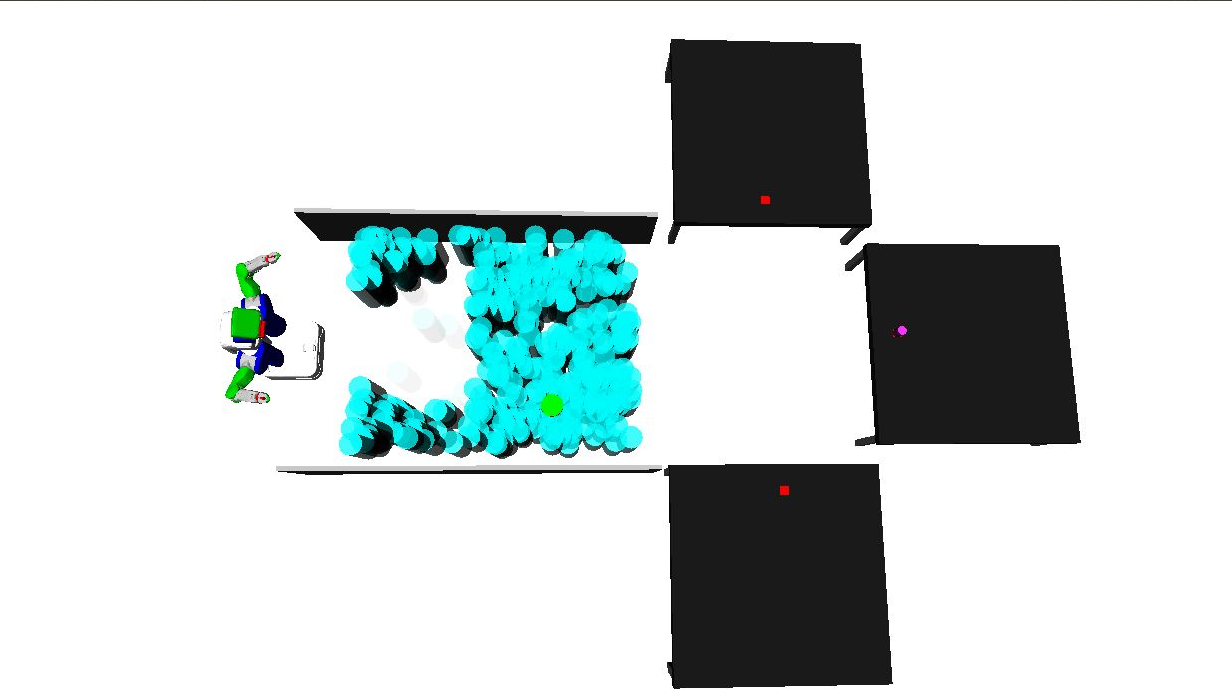
\includegraphics[width=0.45\textwidth]{corridor_images/obj_at_true_loc.png}
  \caption{A screenshot from one of our experiments. The robot is
    tasked with navigating to the other side of the corridor, but
    there is a uniform distribution of obstacles in the way. Our low
    level refinement algorithm detects the probability occlusion and
    propagates information to the high level. The objects shown are
    from the posterior distribution after a single, negative,
    observation. In the rest of the plan, the robot navigates the
    obstruction region, and then searches through the multimodal
    distribution over the goal object, whose true location is shown in pink.}
  \label{fig:knot_steps}
\end{figure}


Discovering a solution to this task necessitates finding a policy that
accounts for uncertainty in locations of objects, locations of the
robot and non-determinism in the dynamics (among other
challenges). Solving such problems exactly is far beyond the state of
the art in partially observable Markov decision processes.

Given the intractability of this problem, how can we hope to make
progress? Our starting point takes inspiration from recent methods for
fully observed task and motion planning.  This is a challenge in its
own right, but careful applications of abstraction, lazy
discretization, and motion planning have made inroads on this
problem~\cite{srivastava2014combined, lozano2014constraint}. These
approaches plan in an \emph{abstract} representation of a problem
(without continuous variables) and use sampling and motion planning to
\emph{refine} abstract plans into fully grounded plans involving continuous
operators.

A key insight is that many of the difficulties in planning with belief
states, which are inherently continuous, are shared by the continuous
state-action spaces for task and motion planning. This suggests a
strategy that applies similar abstraction techniques to belief state
representations of a planning problem.

Another important development is that of \emph{maximum
  likelihood determinizations} (\mld) of
POMDPs~\cite{platt2010belief}. This approximation assumes that each
belief state produces its maximum likelihood observation. The result
is a deterministic problem that encourages reasonable information-gathering
behavior. It is amenable to suitably modified standard
methods; these methods typically prescribe solving a complex,
continuous, under-actuated problem. However, integration with task
planners provides relief from this problem---high level tasks can
split a low-level problem into an observe phase and a motion phase
(which is the output of joint solution methods in many scenarios).

We present an algorithm, Interfaced Belief Space Planning (\ibsp),
that leverages these insights. It extends the domain abstraction techniques from
Srivastava et al.~\cite{srivastava2014combined} to \mld{} formulations of large continuous
POMDPs. We leverage properties of an \mld{} to construct a simple high-level
representation of belief states so that (optimistic) belief
state dynamics are compactly represented. The algorithm alternates
among extracting a plan skeleton, assigning values to continuous
variables, and updating the high level with failure information if a
refinement can not be found.
\ibsp{} enforces a clear separation among extracting plan skeletons
from a domain description, refining a plan skeleton, and determining
success or failure of a plan; furthermore, each component relies on
standard operations. Our implementation uses off-the-shelf classical
planners to generate plan skeletons and sampling and trajectory
optimization to generate refinements. 

Our refinement strategy only requires the ability to compute maximum
likelihood observations for a belief state and the ability to filter
beliefs. We detect plan failure and propose state updates with Monte Carlo
sampling. Such structured access to the belief state allows \ibsp{} to work with a broad class
of beliefs with minimal algorithmic changes. While our high-level
planner uses an abstract belief representation, the full algorithm
plans with the true belief dynamics and is capable of generating and executing plans
with complex state estimation methods. We validate our approach in
partially observable mobile manipulation tasks with a variety of
belief distributions that account for negative observations, such as object retrieval from
one of many possible drawers and navigation through a corridor containing several objects
whose locations are only initially known to be in a uniform distribution over the corridor. We
present formal results showing completeness for a subclass of POMDPs.

%%PA: it'd be really good to include specifics about the
%%scenarios in which we evaluate our approach and specifics about the 
%% behaviors it manages to generate;   for many readers
%%interesting scenarios will make them interested in the approach,
%%lack thereof will make them wonder why they would bother reading
%%this paper...


%%PA: can we have a representative teaser figure on the first page
%%(top of the right column) ?
